\documentclass[a4paper,12pt]{article}
\usepackage[left=1in, right=1in, top=1in, bottom=1in]{geometry}
\usepackage{amsmath, amssymb}
\usepackage{graphicx}
\usepackage{float}
\usepackage{caption}  
\usepackage{subcaption} 
\usepackage{xcolor}
\usepackage{fancyhdr} 
\definecolor{skyblue}{RGB}{135, 206, 235}
\usepackage{wrapfig}
\usepackage{graphicx}

\pagestyle{fancy}
\fancyhf{} % Clear default headers/footers
\fancyhead[R]{\small {CONTINUITY AND DIFFERENTIABILITY \hspace{3mm} 153}} % Right header
\fancyfoot[C]{\small 2019-20} % Centered footer
\renewcommand{\headrulewidth}{0pt} % Remove horizontal line

\begin{document}

    \noindent \textbf{\textcolor{skyblue}{Example 10}}: Discuss the continuity of the function $f$ defined by
    \[
    f(x) =
    \begin{cases} 
    x+2, & \text{if } x \leq 1 \\ 
    x-2, & \text{if } x > 1 
    \end{cases}
    \]

    \noindent \textbf{\textcolor{skyblue}{Solution:}} The function $f$ is defined at all points of the real line.

    \vspace{8pt}
    \noindent \textbf{\textcolor{skyblue}{Case 1:}} If $c < 1$, then $f(c) = c + 2$. Therefore, $\lim\limits_{x \to c} f(x) = \lim\limits_{x \to c} (x + 2) = c + 2$.

    \begin{wrapfigure}{r}{0.4\textwidth}
    \centering
    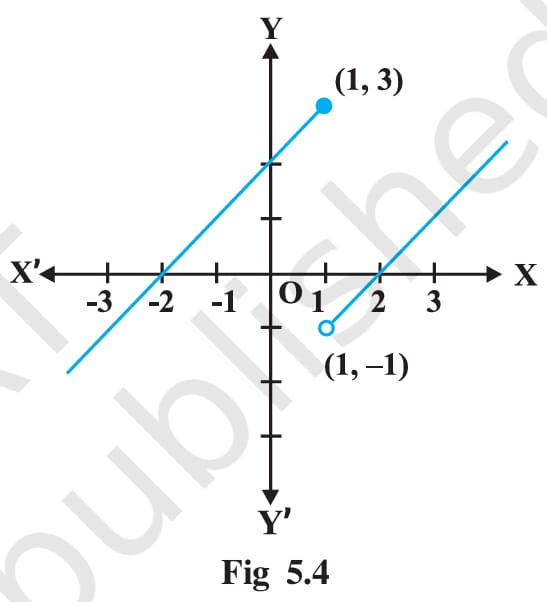
\includegraphics[width=1\linewidth]{a.jpg}
    \end{wrapfigure}
    \noindent Thus, $f$ is continuous at all real numbers less than $1$.
     
    \vspace{4pt}
    \noindent\textbf{\textcolor{skyblue}{Case 2:}} If $c > 1$, then $f(c) = c - 2$. Therefore,
    \[
    \lim\limits_{x \to c} f(x) = \lim\limits_{x \to c} (x - 2) = c - 2 = f(c)
    \]
    Thus, $f$ is continuous at all points $x > 1$.
    \vspace{4pt}
    
    \noindent \textbf{\textcolor{skyblue}{Case 3:}} If $c = 1$, then the left-hand limit of $f$ at $x = 1$ is
    \[
    \lim\limits_{x \to 1^-} f(x) = \lim\limits_{x \to 1^-} (x+2) = 1+2 = 3
    \]
    \noindent The right-hand limit of $f$ at $x = 1$ is
    \[
    \lim\limits_{x \to 1^+} f(x) = \lim\limits_{x \to 1^+} (x-2) = 1-2 = -1
    \]
    \hspace{10pt} Since the left and right-hand limits of $f$ at $x = 1$ do not coincide, $f$ is not continuous at $x = 1$. Hence, $x = 1$ is the only point of discontinuity of $f$.

\vspace{10pt} % Adds space before Example 11

\noindent \textbf{\textcolor{skyblue}{Example 11}}: Find all points of discontinuity of the function $f$ defined by
  \begin{wrapfigure}{r}{0.4\textwidth}
    \centering
    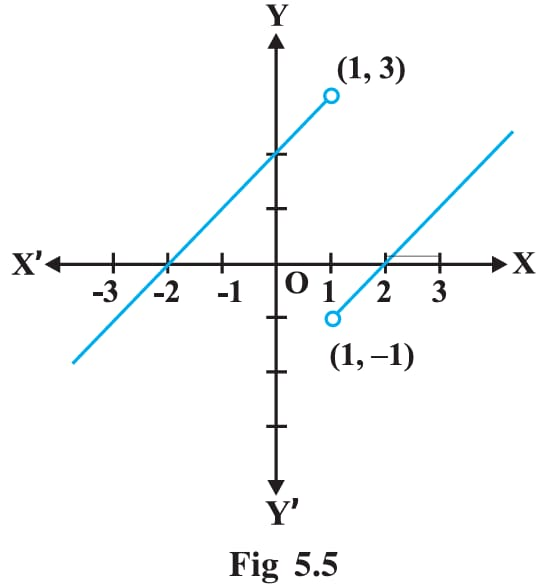
\includegraphics[width=1\linewidth]{b.jpg}
    \end{wrapfigure}

\[
f(x) =
\begin{cases} 
x+2, & \text{if } x < 1 \\ 
0, & \text{if } x = 1 \\ 
x-2, & \text{if } x > 1
\end{cases}
\]

\noindent \textbf{\textcolor{skyblue}{Solution:}} As in the previous example, we find that $f$ is continuous at all real numbers except $x = 1$. The left-hand limit of $f$ at $x = 1$ is
\[
\lim\limits_{x \to 1^-} f(x) = \lim\limits_{x \to 1^-} (x+2) = 1+2 = 3
\]

\noindent The right-hand limit of $f$ at $x = 1$ is
\[
\lim\limits_{x \to 1^+} f(x) = \lim\limits_{x \to 1^+} (x-2) = 1-2 = -1
\]
\hspace{10pt} Since the left and right-hand limits of $f$ at $x = 1$ do not coincide, $f$ is not continuous at $x = 1$. Hence, $x = 1$ is the only point of discontinuity of $f$.The graph of the function is given in the Fig 5.5.

\hfill






\newpage
\pagestyle{fancy}       % Activate fancy header style
\fancyhf{}    
\fancyhead[L]{\small {154 \hspace{3mm}  MATHEMATICS}}
\fancyfoot[C]{\small 2019-20} % Centered footer

\noindent \textbf{\textcolor{skyblue}{Example 12}} Discuss the continuity of the function defined by
\[
f(x) = \begin{cases} 
    x + 2, & \text{if } x < 0 \\
    -x + 2, & \text{if } x > 0
\end{cases}
\]

\noindent \textbf{\textcolor{skyblue}{Solution:}} Observe that the function is defined at all real numbers except at $0$.

\begin{wrapfigure}{r}{0.4\textwidth}
    \centering
    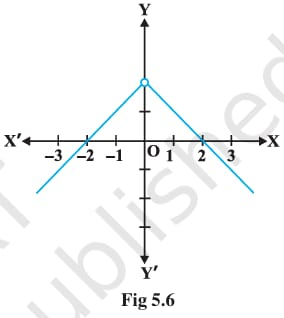
\includegraphics[width=1\linewidth]{c.jpg}
    \vspace{-2cm}
\end{wrapfigure}
\hspace{-2cm}

\noindent Domain of definition of this function is
\[
\hspace{0cm}
\begin{aligned}
    D_1 \cup D_2 & \quad \text{where} \quad D_1 = \{x \in \mathbb{R} : x < 0\} \quad and  \\
                 & \quad \quad \quad \quad \hspace{2mm} D_2 = \{x \in \mathbb{R} : x > 0\}
\end{aligned}
\]

\noindent \textbf{\textcolor{skyblue}{Case 1:}} If $c \in D_1$, then  
$\lim\limits_{x \to c} f(x) = \lim\limits_{x \to c} (x+2)$ \\
\vspace{4pt}
\noindent = $c$ + 2 = $f(c)$ and hence $f$ is continuous in $D_1$.

\vspace{4pt}
\noindent \textbf{\textcolor{skyblue}{Case 2:}} If $c \in D_2$, then
$\lim\limits_{x \to c} f(x) = \lim\limits_{x \to c} (-x + 2)$ \\
\vspace{4pt}
= -c + 2 = f(c) and hence, $f$ is continuous in $D_2$.\\ Since $f$ is continuous at all points in the domain of $f$,  we deduce that f is continuous. Graph of this
 function is given in the Fig 5.6. Note that to graph
 this function we need to lift the pen from the plane
 of the paper, but we need to do that only for those points where the function is not
 defined.

\vspace{10pt} % Adds space before Example 13

\noindent \textbf{\textcolor{skyblue}{Example 13}} Discuss the continuity of the function $f$ given by

\begin{wrapfigure}{r}{0.4\textwidth}
    \centering
    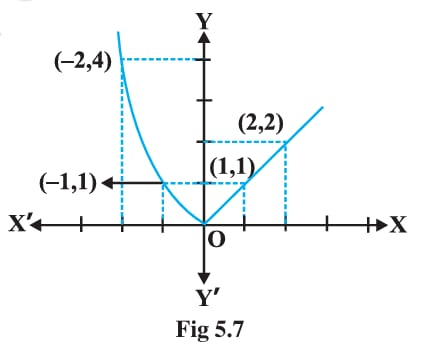
\includegraphics[width=1\linewidth]{d.jpg}
    \vspace{-1cm}
\end{wrapfigure}
\hspace{-3cm}

\noindent \[
\hspace{0cm}
f(x) = \begin{cases} 
    x, & \text{if } x \geq 0 \\
    x^2, & \text{if } x < 0
\end{cases}
\]

\noindent \textbf{\textcolor{skyblue}{Solution:}} Clearly the function is defined at every real number. Graph of the function is given in Fig 5.7. By inspection, it seems prudent to partition the domain of definition of  into three disjoint subsets of the real line.
\vspace{-6pt}

\[
\begin{aligned}
    \text{Let} \quad D_1 &= \{x \in \mathbb{R} : x < 0\}, \quad D_2 = \{0\} \quad and \\
    D_3 &= \{x \in \mathbb{R} : x > 0\}
\end{aligned}
\]

\noindent \textbf{\textcolor{skyblue}{Case 1:}} At any point in D1
 , we have $f(x)$ = $x^2$ and it is easy to see that it is continuous
 there (see Example 2).  \hfill

\noindent \textbf{\textcolor{skyblue}{Case 2:}} At any point in D3
 , we have $f(x)$ = $x$ and it is easy to see that it is continuous
 there (see Example 6). \hfill

\noindent \textbf{\textcolor{cyan}{Case 3}} Now we analyse the function at \( x = 0 \). The value of the function at 0 is \( f(0) = 0 \). The left-hand limit of \( f \) at \( 0 \) is
\[
\lim_{x \to 0^-} f(x) = \lim_{x \to 0^-} x^2 = 0^2 = 0
\]

The right-hand limit of \( f \) at \( 0 \) is
\[
\lim_{x \to 0^+} f(x) = \lim_{x \to 0^+} x = 0
\]

\end{document}
